\documentclass{article}
\usepackage{amsmath}
\usepackage{amsthm}
\usepackage{amsfonts}
\usepackage{amssymb}
\usepackage{bbold}
\usepackage{dsfont}
\usepackage{graphicx}
\usepackage{cleveref}
\usepackage{bm}
\usepackage{booktabs}
\usepackage{siunitx}
\usepackage{xcolor}
\usepackage{pdfpages}
\usepackage[utf8]{inputenc}
\usepackage[english]{babel}
\newtheorem{definition}{Definition}
\newtheorem{example}{Example}
\newcommand{\exP}[1]{\mathrm{e}^{#1}}
\newcommand{\dif}{\mathrm{d}}
\renewcommand{\vec}[1]{\mathbf{#1}}
\newcommand{\pdagger}{{\phantom{\dagger}}}
\newcommand{\state}[1]{\vert #1\rangle}
\newcommand{\cstate}[1]{\langle #1\vert}
\newcommand{\tr}[1]{\mathrm{tr}\left\{#1\right\}}
\newcommand{\trs}[2]{\, \mathrm{tr}_{#1}\{#2\}}
\newcommand{\expc}[3]{\langle #1\vert #2 \vert #3\rangle}
\usepackage[doi=false,url=false,isbn=false,backend=bibtex,style=nature,natbib=true,sorting=none]{biblatex}
\bibliography{bib.bib}
\usepackage{geometry}
\geometry{
	a4paper,
	total={170mm,257mm},
	left=15mm,
	right=15mm,
	top=15mm,
}
\begin{document}
\title{Report 1: Spin mapping for singlet fission dynamics project}
\author{Rudolf Smorka}
\maketitle
\section{Equations of motion}
Within the spin mapping approach, one obtains the equations of motion  
\begin{align}
	\frac{\dif Z_\lambda}{\dif t} &= -i \sum_\mu \langle \lambda \vert \hat{V}(x)\vert \mu\rangle Z_\mu\label{eq:EOM_1}\\
	\frac{\dif x}{\dif t} &= \frac{p}{m}\label{eq:EOM_2}\\
	\frac{\dif p}{\dif t} &=F_0(x) +F_e(\mathcal{Z},\mathcal{Z}',x),\label{eq:EOM_3}
\end{align}
where $Z_\lambda= X_\lambda+ iP_\lambda$ are cartesian mapping variables for the electronic system, combined all together in the set of all mapping variables $\mathcal{Z}=\{Z_1,\dots,Z_F\}$, and $x$ and $p$ are the classical positions and momenta of the oscillators. In the equation of motion of the mapping variables, $\hat{V}(x)$ is the traceless electron-nuclear coupling operator. 
Further, $F_0(x)$ and $F_e(\mathcal{Z},x)$ are the nuclear forces corresponding to the state-independent potential $V_0(x)$ and the mapped electron-nuclear coupling $V_m(\mathcal{Z})$, respectively
\begin{align*}
	F_0(x) &= -\nabla V_0(x),\\
	F_e(\mathcal{Z},\mathcal{Z}',x) &= -\frac{\nabla}{2}( V_m(\mathcal{Z}) + V_m(\mathcal{Z}')).
\end{align*} 
\section{Integrators}
In order to evaluate observables based on the spin-PLDM correlation function, one propagates numerically \cref{eq:EOM_1,eq:EOM_2,eq:EOM_3}, where $\mathcal{Z}$ and $\mathcal{Z}'$ are treated equally.
Previously, there were two integrators implemented in the spin-PLDM code, namely, one based on lsoda\footnote{lsoda is a method that switches between the linear multistep/Adams method and the backward differentiation method depending on an automatic stiffness detection.} from the Fortran library odepack, and an integrator which does both an exact step in the electronic and nuclear EOM, described in Ref.~\cite{richardson2017analysis}. In practice, the former integrator converges poorly for high dimensional problems, while the latter is available only for harmonic frequencies which are the same in all electronic states. As the model of o-TIPSPm built in Ref.~\cite{reddy2018intramolecular} is of a vibronic coupling type containing modes with differing frequencies, this integrator will lead to wrong results.
Recently, another integrator has been implemented which performs an exact update for the electronic degrees of freedom but a velocity-verlet step in the nuclear degrees of freedom. The performance of that integrator is compared in the following. 
\section{Comparison of integrators for a single trajectory}
For the following comparison a single realization of $\mathcal{Z}(t_0)$ and $x(t_0),p(t_0)$ has been propagated using the lsoda integrator as implemented in odeint and was compared to the recently implemented velocity-verlet one.
\Cref{fig:Comp_single_S0S1} shows the population dynamics of the locally excited (LE) state $\vert S_0S_1\rangle $, which is occupied initially, and \cref{fig:Comp_single_T1T1} the dynamics of the multiexcitonic (ME) state $\vert T_1T_1\rangle$, that is a correlated triplet pair state.
Therein, the red line is the integration using odeint, the black full, blue and green dashed lines are obtained using a velocity-verlet algorithm with different time steps (the legends show time-steps in a.u.). 
The first check is for which the results converge with varying time step. Since an adaptive time step is using in the odeint integrator, we do not show a fixed $dt$ in the plots below. All lines agree well for times, depending on the time-step in the velocity verlet integrator. As expected, the deviation decreases with decreasing time step. 
\begin{figure}[!h]
	\centering
	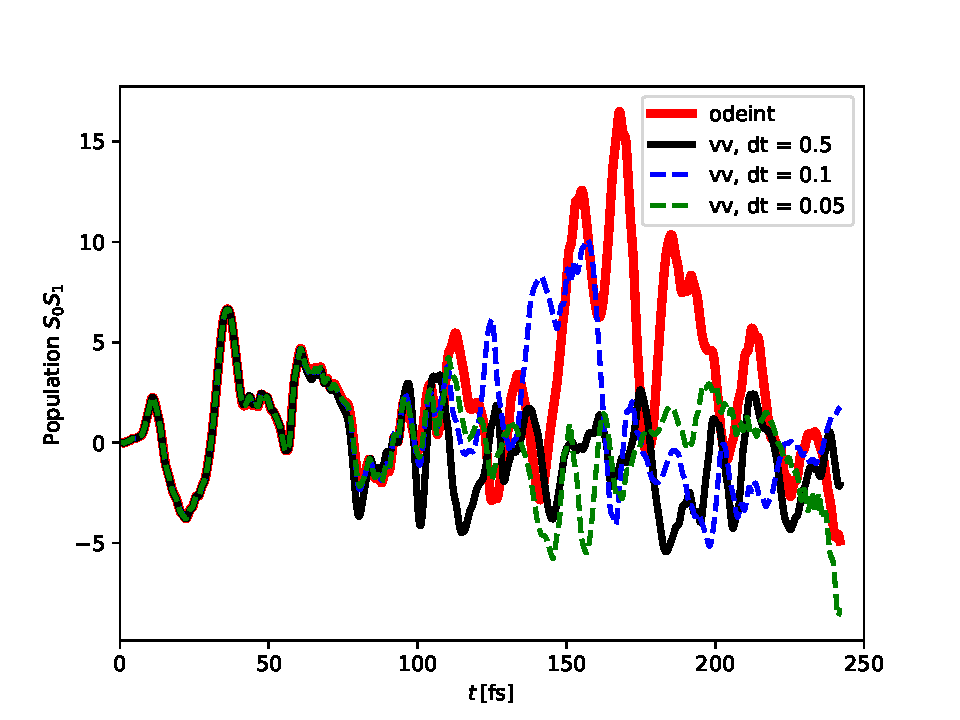
\includegraphics[width=0.6\textwidth]{figs/SF_comparison_single_traj_S0S1.pdf}
	\caption{Comparison of the time evolution of the singly locally excited state (single trajectory).}\label{fig:Comp_single_S0S1}
\end{figure} 
\begin{figure}[!h]
	\centering
	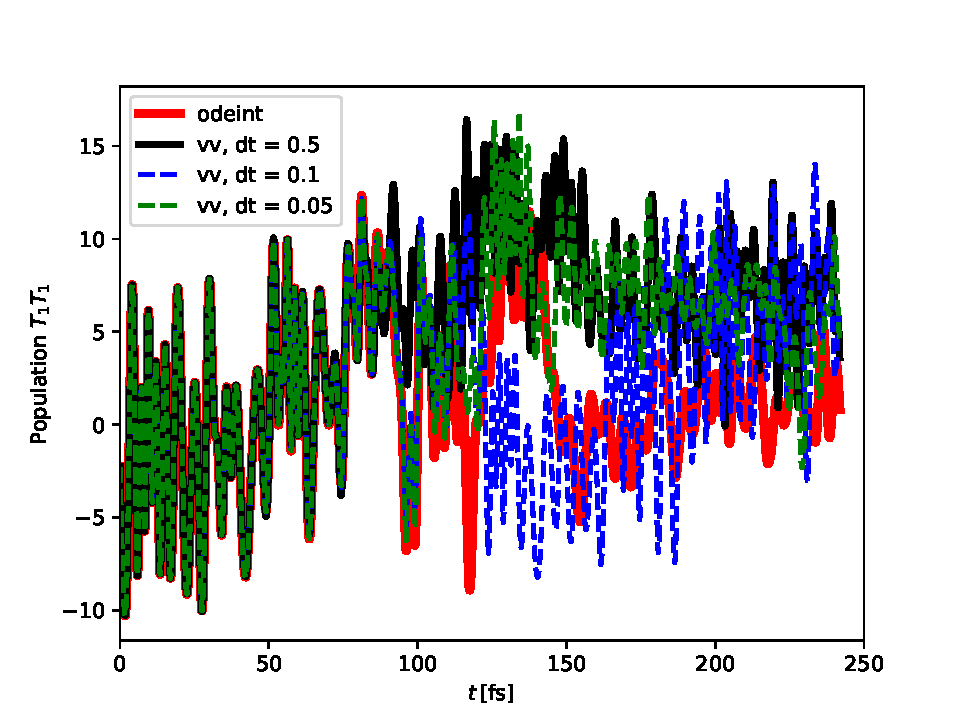
\includegraphics[width=0.6\textwidth]{figs/SF_comparison_single_traj_T1T1.pdf}
	\caption{Comparison of the time evolution of the multiexcitonic triplet pair state (single trajectory).}\label{fig:Comp_single_T1T1}
\end{figure}
\clearpage
\section{Convergence with number of trajectories}
We now turn to the multi-trajectory averaged results. 
First, we investigate how many trajectories are necessary in order for the electronic populations to be converged. Here, we employ the velocity-verlet step for the nuclear DoF and the exact matrix exponential step for the electronic DoF. \Cref{fig:Comp_conv_multi_traj_S0S1,fig:Comp_conv_multi_traj_T1T1} show the dynamics of the LE and the ME states, respectively. The time step is fixed to  $dt=0.5\, \mathrm{a.u.}\doteq \SI{0.012}{\femto\second}$. Therefore, the results are expected to be converged approximately up to $\SI{100}{\femto\second}$ with respect to the time-step, assuming the odeint integrator leads to correct results. The population dynamics, both for $n_\mathrm{traj}=10^6$ and $n_\mathrm{traj}=3\cdot 10^6$ trajectories, agree  very well.  
However, these results show two significant problems: First, the initial populations deviate strongly from the expected ones. 
The second problem is that trajectory-averaged populations become unphysical temporarily. On a single-trajectory level, this is to be expected within the spin mapping approach.
\begin{figure}[!h]
	\centering
	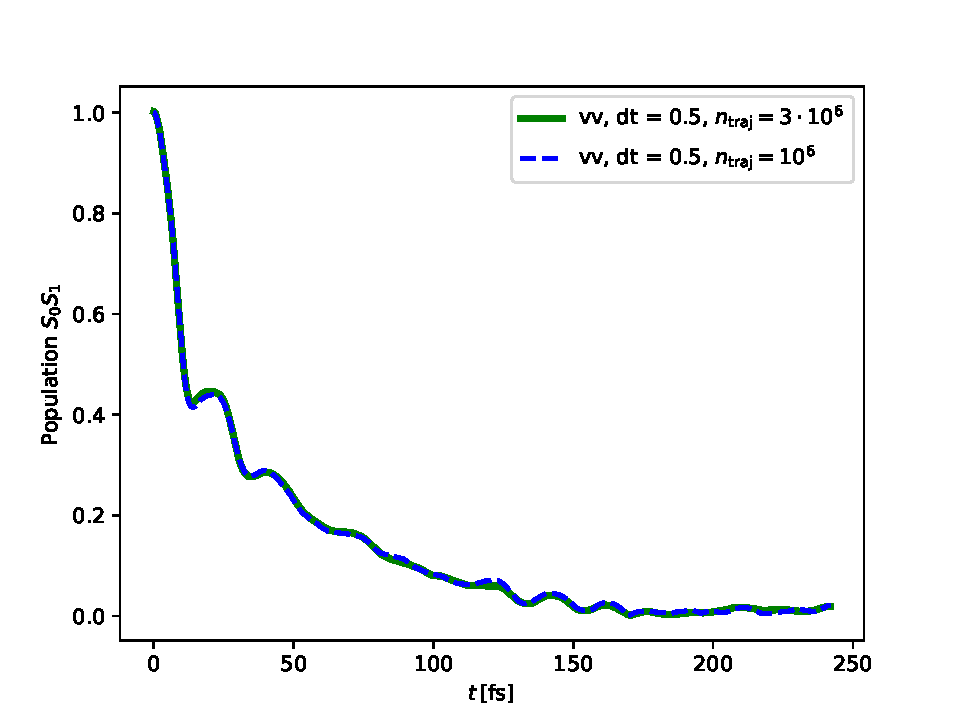
\includegraphics[width=0.6\textwidth]{figs/SF_comparison_multi_vv_traj_S0S1.pdf}
	\caption{Comparison of the time evolution of the singly locally excited state.}\label{fig:Comp_conv_multi_traj_S0S1}
\end{figure} 
\begin{figure}[!h]
	\centering
	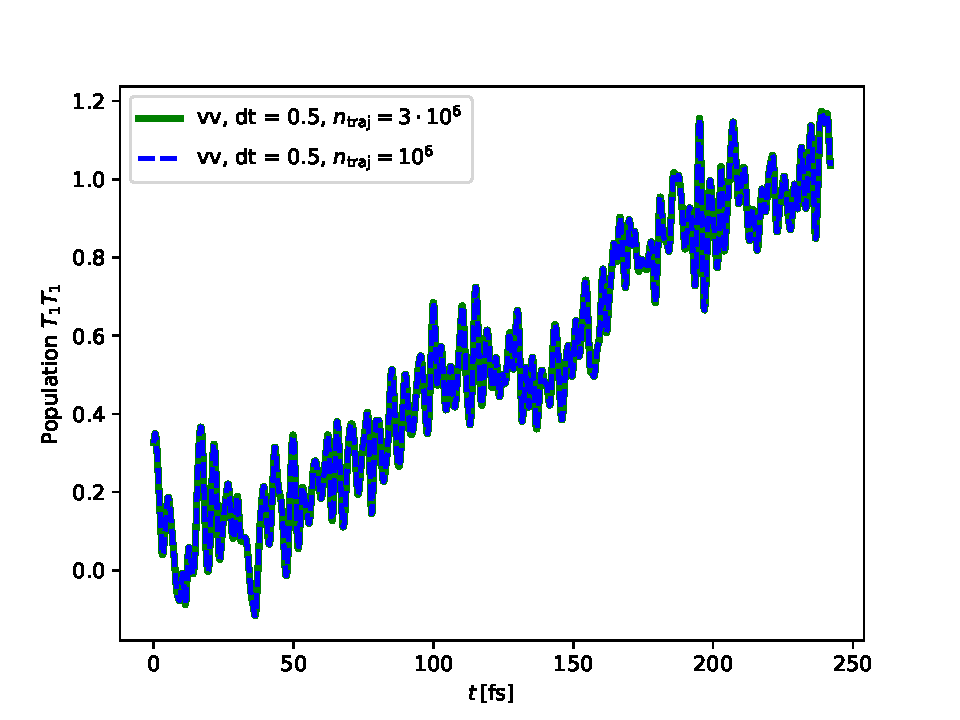
\includegraphics[width=0.6\textwidth]{figs/SF_comparison_multi_vv_traj_T1T1.pdf}
	\caption{Comparison of the time evolution of the multiexcitonic triplet pair state.}\label{fig:Comp_conv_multi_traj_T1T1}
\end{figure}
\clearpage
\section{Comparison of integrators: Multitrajectory results}
After determining the sufficient number of trajectories and time step in order to obtain converged results, one can compare the performance of the velocity verlet integrator against the odeint method. The populations dynamics of the LE and ME states are shown in \cref{fig:Comp_multi_S0S1,fig:Comp_multi_T1T1}, respectively. Therein we also show ML-MCTDH results as published in Ref.~\cite{reddy2018intramolecular}. 
The agreement between the spin-PLDM approach (both odeint method and velocity verlet integrator) with the ML-MCTDH results, unfortunately, is very poor for the shown time steps and number of trajectories. 
In particular this comparison clearly shows that the trajectory-averaged velocity verlet results are not fully converged with respect to the time step, even for very short times.  
\begin{figure}[!h]
	\centering
	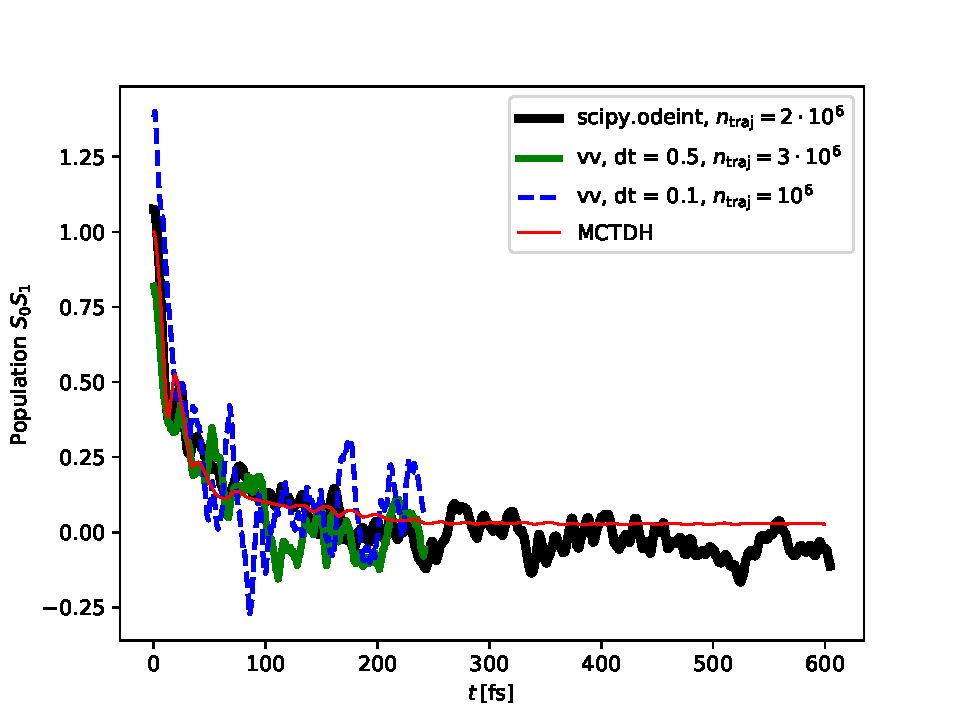
\includegraphics[width=0.6\textwidth]{figs/SF_comparison_multi_S0S1.pdf}
	\caption{Comparison of the time evolution of the singly locally excited state.}\label{fig:Comp_multi_S0S1}
\end{figure} 
\begin{figure}[!h]
	\centering
	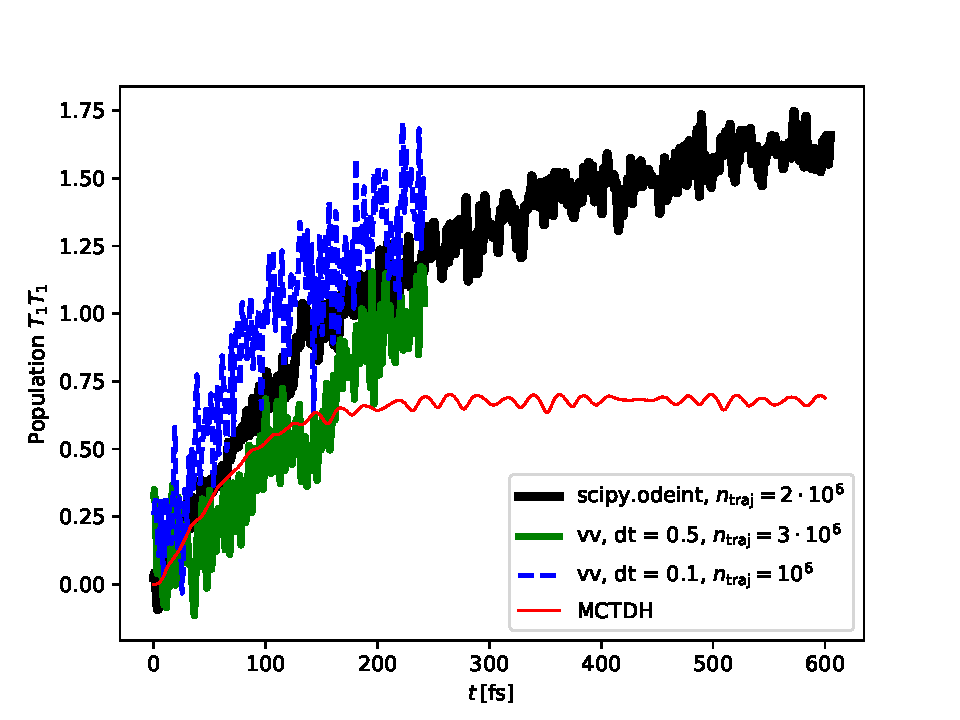
\includegraphics[width=0.6\textwidth]{figs/SF_comparison_multi_T1T1.pdf}
	\caption{Comparison of the time evolution of the multiexcitonic triplet pair state.}\label{fig:Comp_multi_T1T1}
\end{figure}

\section{To do}
The comparison between $10^6$ and $3\cdot 10^6$ indicates that $10^6$ trajectories is sufficient in order to obtain converged results. Computations are currently running for time steps  $\SI{1.2}{\atto\second}$, $\SI{0.24}{\atto\second}$ and $\SI{0.12}{\atto\second}$. 

\printbibliography
\end{document}


